\documentclass{beamer}
\usepackage{ctex, hyperref}
\usepackage[T1]{fontenc}
\usepackage[numbers.sort]{natbib}

% other packages
\usepackage{latexsym,amsmath,xcolor,multicol,booktabs,calligra}
\usepackage{graphicx,pstricks,listings,stackengine}

\author{卢韬 \textrm{20194127}}
\title{专业外语演讲}
\subtitle{\textrm{Object Detection}}
\institute{自动化1903}
\date{\today}
\usepackage{SudaBeamer}



% defs
\def\cmd#1{\texttt{\color{red}\footnotesize $\backslash$#1}}
\def\env#1{\texttt{\color{blue}\footnotesize #1}}
\definecolor{deepblue}{rgb}{0,0,0.5}
\definecolor{deepred}{rgb}{0.6,0,0}
\definecolor{deepgreen}{rgb}{0,0.5,0}
\definecolor{halfgray}{gray}{0.55}

\lstset{
    basicstyle=\ttfamily\small,
    keywordstyle=\bfseries\color{deepblue},
    emphstyle=\ttfamily\color{deepred},    % Custom highlighting style
    stringstyle=\color{deepgreen},
    numbers=left,
    numberstyle=\small\color{halfgray},
    rulesepcolor=\color{red!20!green!20!blue!20},
    frame=shadowbox,
}


\begin{document}

% \setcitestyle{notesep={; },round,aysep={},yysep={;}}


\kaishu
% \setmainfont{Times New Roman}   face-challenge.png
\begin{frame}
    \titlepage
    \begin{figure}[htpb]
        \begin{center}
            
\includegraphics[width=0.2\linewidth]{pic/Suda_Log.png}
        \end{center}
    \end{figure}
\end{frame}

\begin{frame}
    \tableofcontents[sectionstyle=show,subsectionstyle=show/shaded/hide,subsubsectionstyle=show/shaded/hide]
\end{frame}


\section{Object Detection}

\begin{frame}{Recognition by Computers}
    \begin{itemize}[<+-| alert@+>] % 当然,除了alert,手动在里面插 \pause 也行
        \item %Since 1950, when computer vision just emerge as an psychological method, the task of recognition has been studied for many years. 
       \centering “What objects are where?”
    \end{itemize}
    
    \begin{figure}[h!]
        \begin{center}
            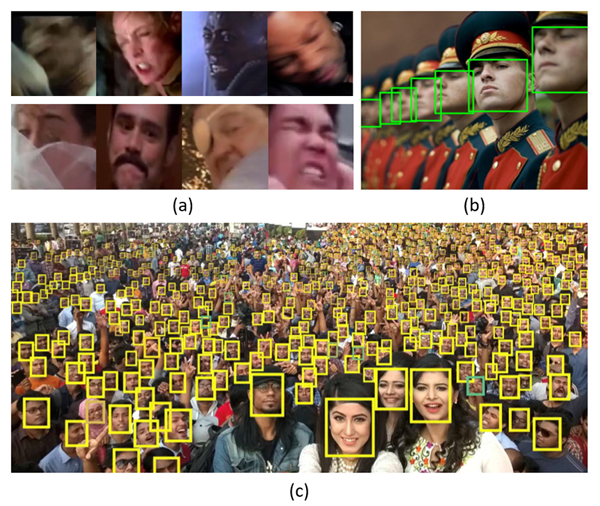
\includegraphics[width=0.55\linewidth]{face-challenge.png}
            \caption{Challenges in face detection: (a) Intra-class variation, image from WildestFaces Dataset . (b) Face occlusion, image from UFDD Dataset .  (c) Multi-scale face detection. Image from \textit{P. Hu et al.\ CVPR2017}
            }
        \end{center}
    \end{figure}    
    
    \begin{figure}[h!]
        \begin{center}
            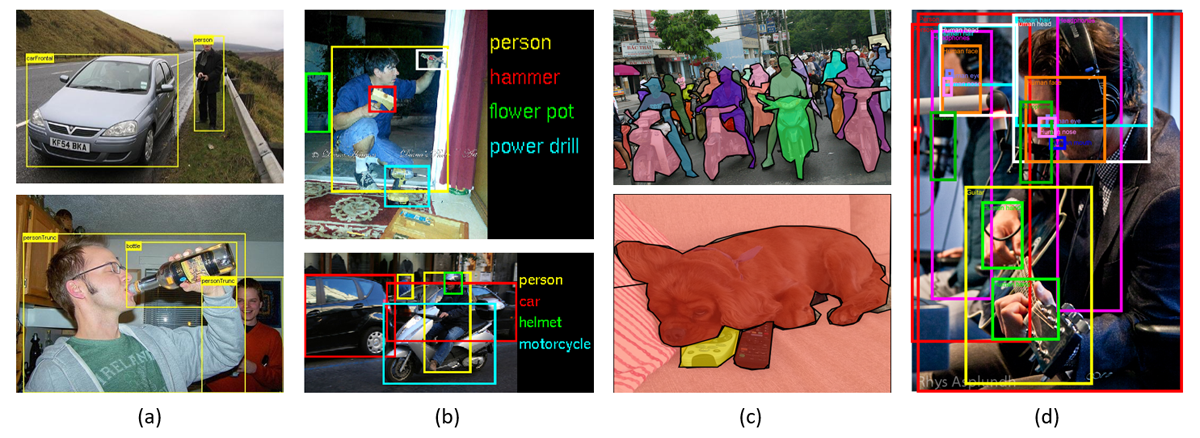
\includegraphics[width=1\linewidth]{dataset-examples.png}
            \caption{Some example images and annotations in (a) PASCAL-VOC07, (b) ILSVRC, (c) MS-COCO, and (d) Open Images.}
        \end{center}
    \end{figure}
    
\end{frame}


\begin{frame}
    \begin{itemize}[<+-| alert@+>]
        \item Object detection, as of one the most fundamental and challenging problems in computer vision, has received great attention in recent years. 
        \item Its development in the past two decades can be regarded as an epitome of computer vision history. 
       \begin{figure}[h!]
                \begin{center}
                    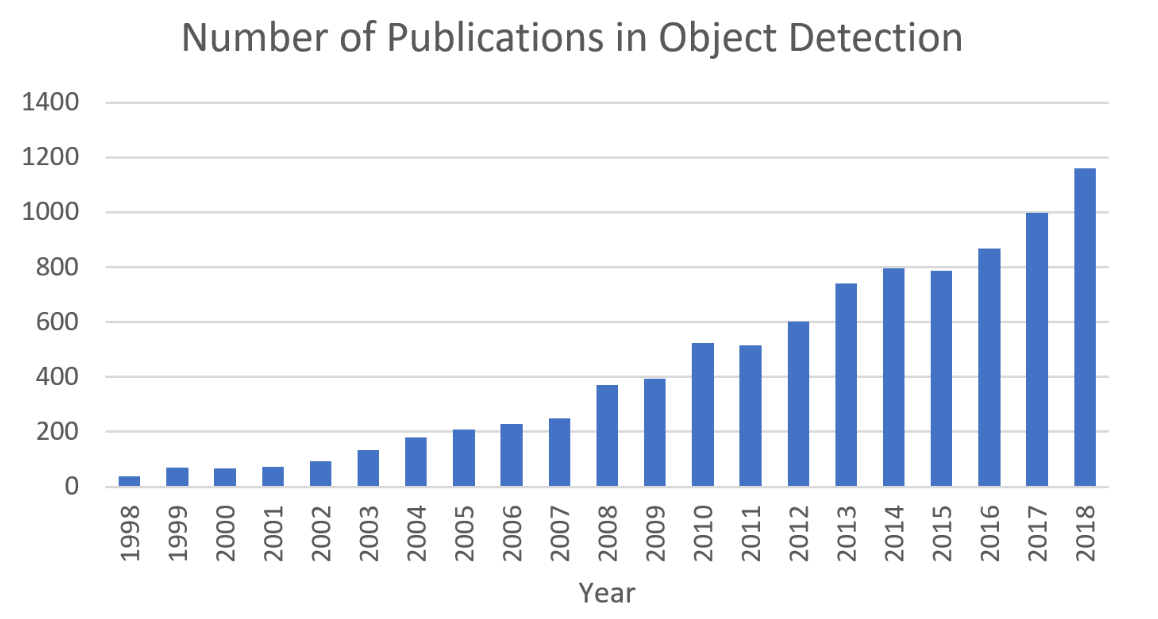
\includegraphics[width=0.7\linewidth]{number-of-papers.png}
                    \caption{\small The increasing number of publications in object detection from 1998 to 2018. (Data from Google scholar advanced search: \textit{allintitle: ``object detection'' AND ``detecting objects''}.)}
                \end{center}
        \end{figure}
        
    \end{itemize}

\end{frame}
%        
\begin{frame}
    \begin{itemize}
        \item If we think of today's object detection as a technical aesthetics under the power of deep learning, then turning back the clock 20 years we would witness the wisdom of cold weapon era. 
        \begin{figure}[h!]
            \begin{center}
                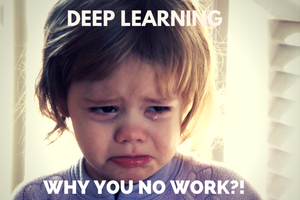
\includegraphics[width=0.7\linewidth]{memedeeplearning.png}
                \caption{\small When Deep Learning does not work.}
            \end{center}
        \end{figure}
        
    \end{itemize}
\end{frame}


\begin{frame}
    \begin{itemize}
        \item As is known to us all, detectors, datasets and metrics take the essential roles in deep learning based methods. 
        \item And it is the framework of the detectors that really counts. 
        \item So in my speech, I will demonstrate the history of the legacy milestone detectors. 
        
    \end{itemize}
\end{frame}

\begin{frame}
    \begin{itemize}
        \item As is shown in this figure it is what happened during the past two decades. 
        \begin{figure}[h!]
            \begin{center}
                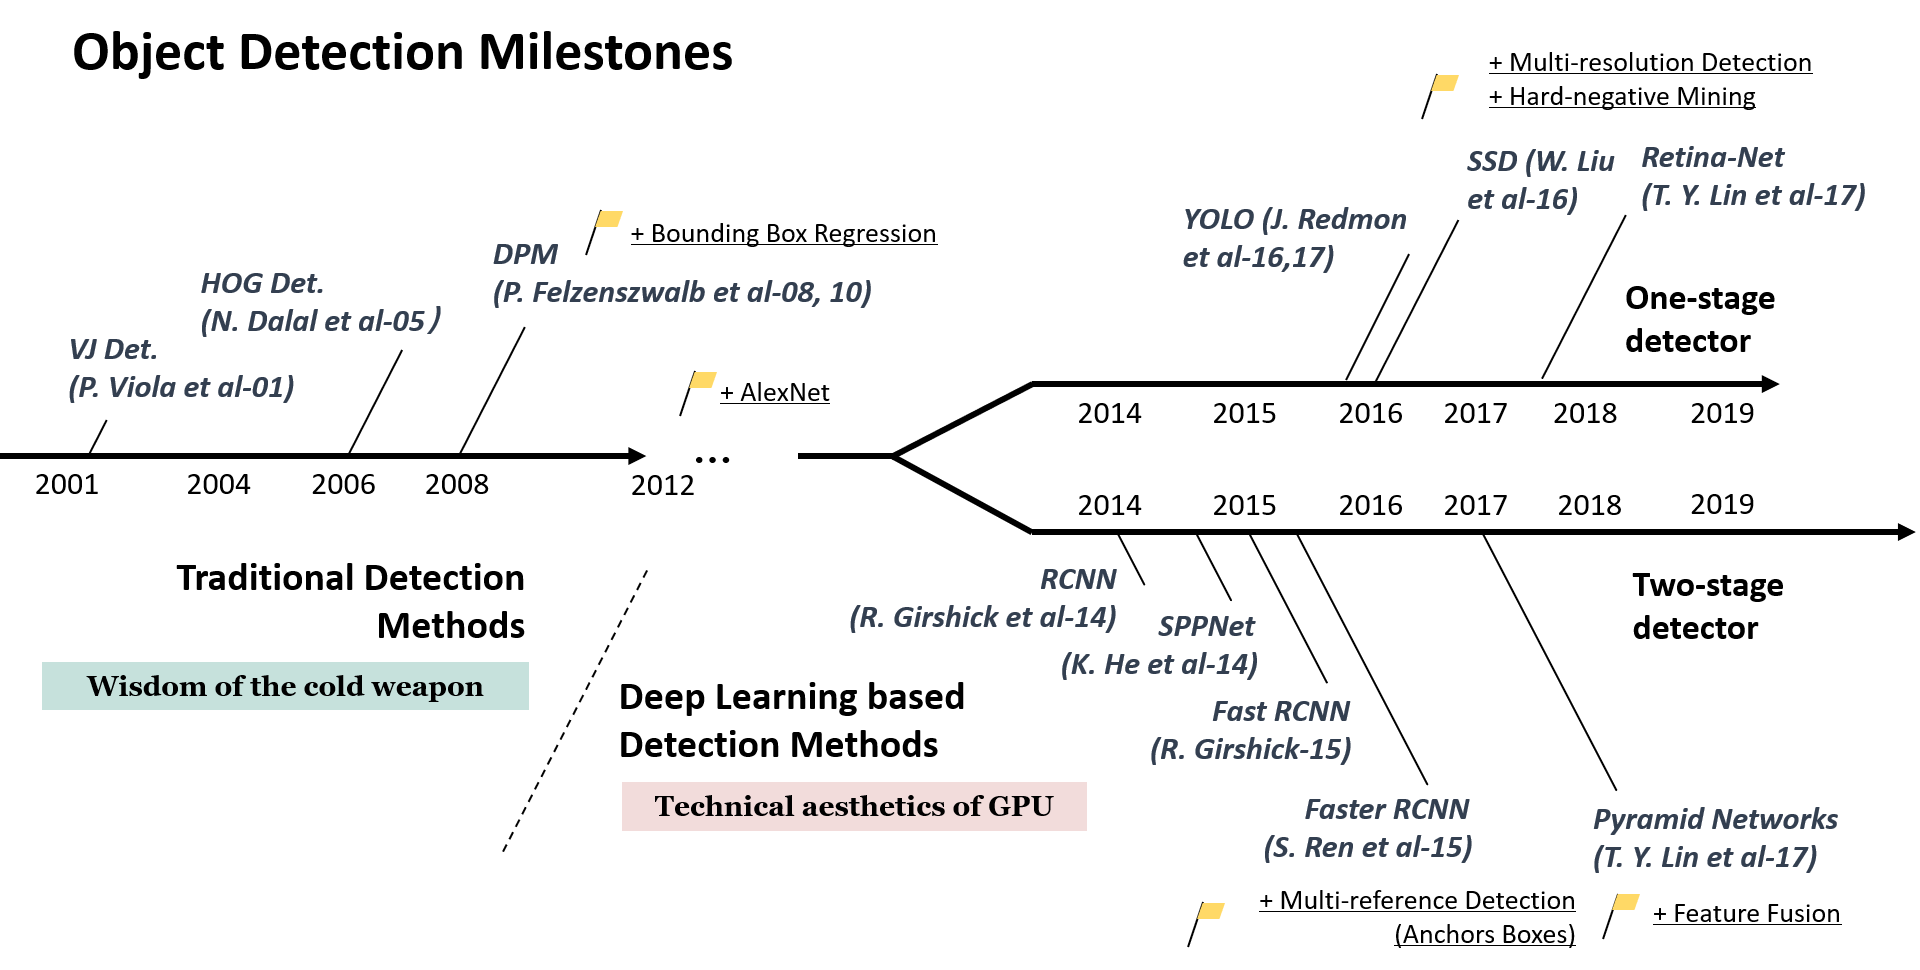
\includegraphics[width=0.99\linewidth]{mile-stones.png}
                \caption{\small  A road map of object detection.}
            \end{center}
        \end{figure}
    
    % 自己说的
       % \item If you have read some papers regarding this field, or its downstream application, like face detection or pedestrian detection, you must be familiar with several key words, like RCNN, its Fast version, and the Faster one. 
        
    \end{itemize}
\end{frame}


\section{Classical}
\begin{frame}
    \begin{itemize}[<+-| alert@+>]
        \item Although it seems to be a very simple process, the calculation behind it was far beyond the computer's power of its time. \begin{figure}[h!]
            \begin{center}
                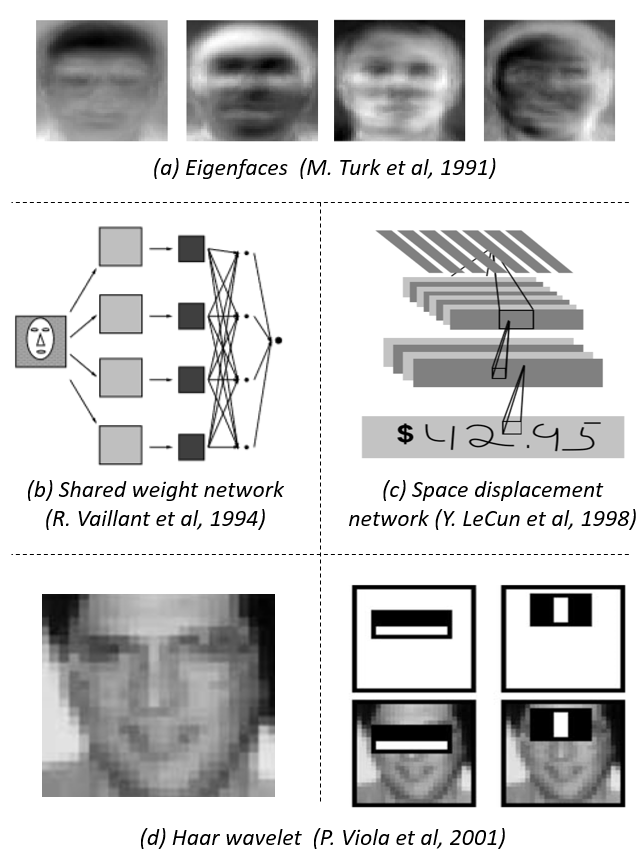
\includegraphics[width=0.4\linewidth]{earlytime.png}
                \caption{\small Some well-known detection models of the early time: (a) Eigenfaces , (b) Shared weight networks , (c) Space displacement networks (Lenet-5) , (d) Haar wavelets of VJ detector}
            \end{center}
        \end{figure}
 
    \end{itemize}

\end{frame}
%        
\begin{frame}
    \begin{itemize}[<+-| alert@+>]
        \item The VJ detector has dramatically improved its detection speed by incorporating three important techniques: ``integral image'', ``feature selection'', and ``detection cascades''. 
        \item It requires optimization techniques , computational optimization tricks and many handcrafted features.
        \begin{figure}[h!]
            \begin{center}
                
\includegraphics[width=0.4\linewidth]{memehandcraft.png}
                \caption{\small Statistical learning}
            \end{center}
        \end{figure}
    \end{itemize}

\end{frame}

\begin{frame}{HOG}
    \begin{itemize}
        \item Years later, HOG brings out scale-invariant feature transform and shape contexts. 
        \item Although it is descned for person Reid, its detector has long been an important foundation of many object detectors 
        \tiem and a large variety of computer vision applications for many years.
    \end{itemize}
\end{frame}




\section{Two-stage}
\begin{frame}
    \begin{itemize}
        \item 2012 is the milestone for CNN, when Alex proposed AlexNet\cite{alexnet}.
        \item A deep convolutional network is able to learn robust and high-level feature representations of an image. 
        \item In deep learning era, object detection can be grouped into two genres: 
        “two-stage detection” and “one-stage detection”, 
        where the former frames the detection as a “coarse-to-fine” process 
        while the later frames it as to “complete in one step”.
    \end{itemize}
\end{frame}

\subsection{NOT end to end}

\begin{frame}
    \begin{itemize}
        \item Then in 2014, RCNN used a CNN by proposing the Regions and brought the deep learning era for object detection.
        \item Later in that year, SPPNet\cite{sppnet} proposed Spatial Pyramid Pooling to share the convolutional features.
        \item In 2015,  Fast RCNN\cite{fast} combined SPP and RCNN and made inference cost efficiently. 
    \end{itemize}
\end{frame}

\subsection{end to end}

\begin{frame}
    \begin{itemize}
        \item Soon, Faster RCNN\cite{faster} used a RPN neck to realized the first end to end training pipline. 
        \begin{figure}[h!]
            \begin{center}
                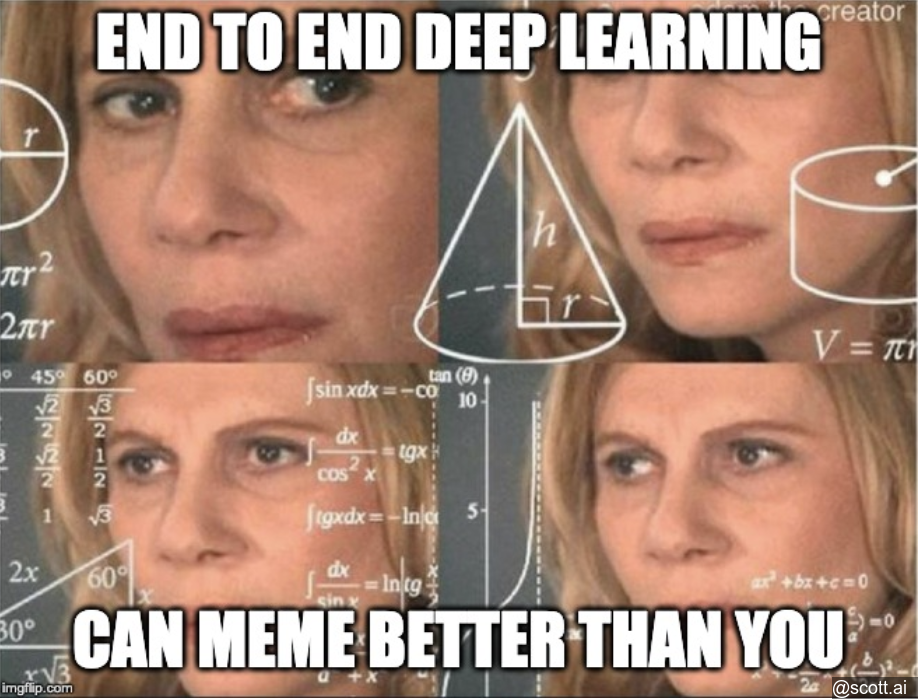
\includegraphics[width=0.5\linewidth]{memeendtoend.png}
                \caption{\small End to end learning}
            \end{center}
        \end{figure}
        
        \item In 2017, FPN\cite{fpn} proposed Feature Pyramid to detect objects with a wide variety of scales. 
    \end{itemize}
\end{frame}


\section{One-stage}


% \subsection{如何更好地做Beamer}

\begin{frame}[<+-| alert@+>]{YOLO}
    \begin{itemize}
        \item YOLO was the first one-stage detector in deep learning era.
            \begin{figure}
                \centering
                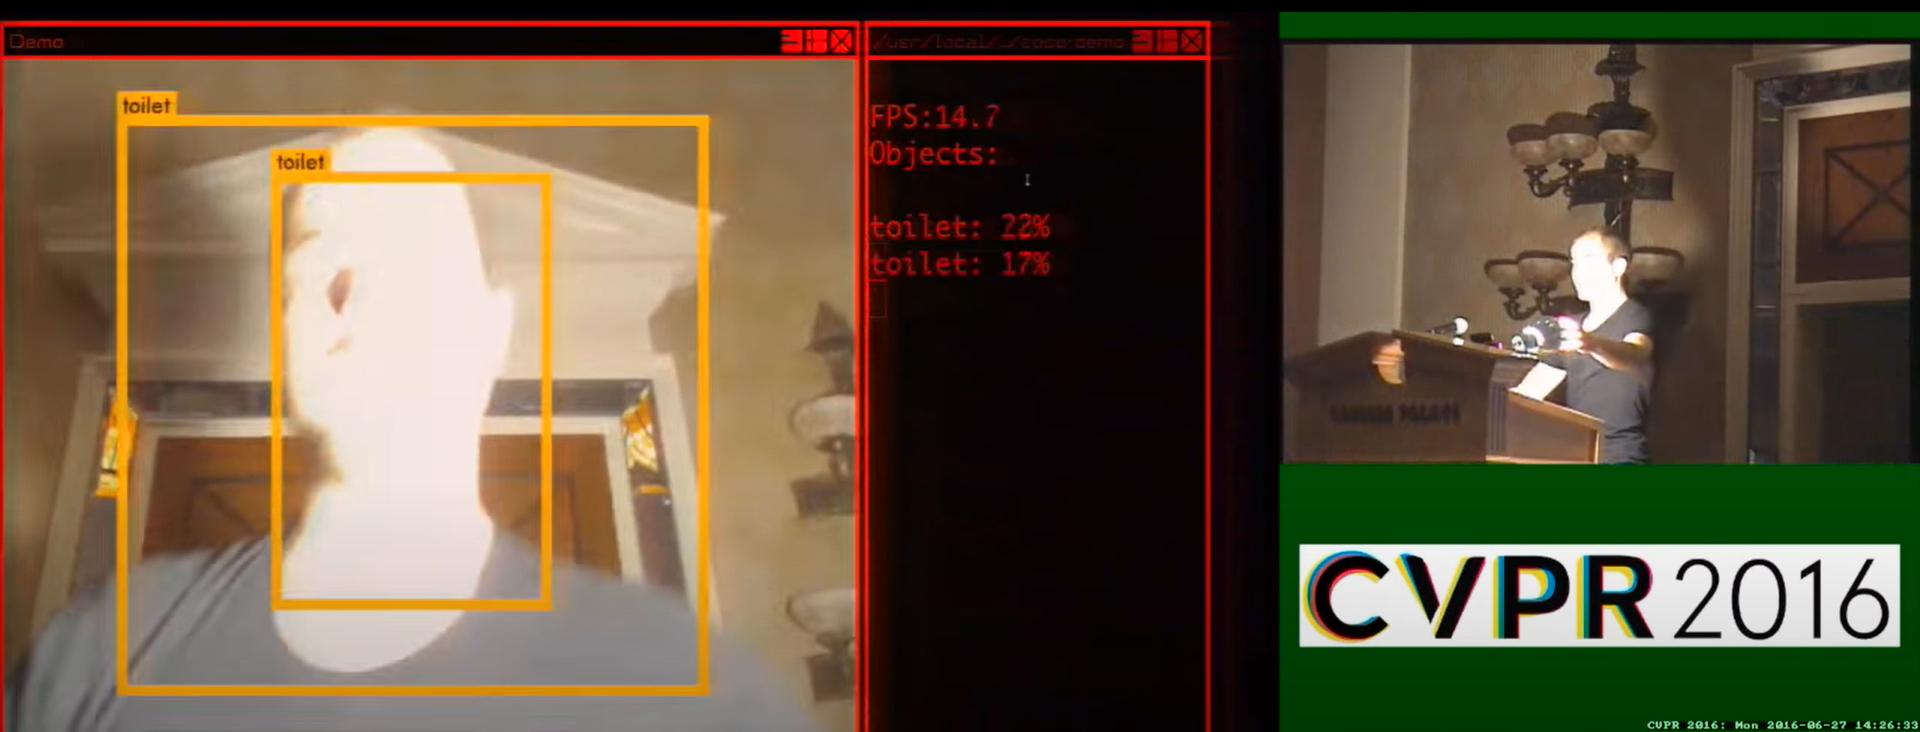
\includegraphics[width=1\linewidth]{yolo.png}
                \caption{YOLO speech: “They rally think white shining things are toilets”}
                \label{fig:my_label}
            \end{figure}
        \item Its first version\cite{yolo} was published in 2015,
        \item and the second version\cite{yolo9000} in 2017,
        \item followed by the third version\cite{yolov3} in 2018.
        
        % \item 
    \end{itemize}
    
\end{frame}

\begin{frame}[<+-| alert@+>]
    \begin{itemize}
        \item Also in 2015, SSD introduced the multi-scale technique and had advantages in terms of both detection speed and accuracy.
        \item  In 2017, RetinaNet used focal loss to handle class imbalance caused by dataset.
        \begin{equation}
            L(y, \hat{p})
= -\alpha y \left(1 - \hat{p}\right)^\gamma \log(\hat{p})
- (1 - y) \hat{p}^\gamma \log(1 - \hat{p})
        \end{equation}
    
    \item Mask R-CNN
        
    \end{itemize}
    
\end{frame}
  













\section{Conclusion}

\begin{frame}{}

Remarkable achievements have been made in object detection over the past 20 years. Although a great effort has been made in recent years, the speed gap between a machine and human eyes still remains large, especially for detecting some small objects. With many open questions unsolved, the field of object detection still needs your help.
        \begin{figure}
                \centering
                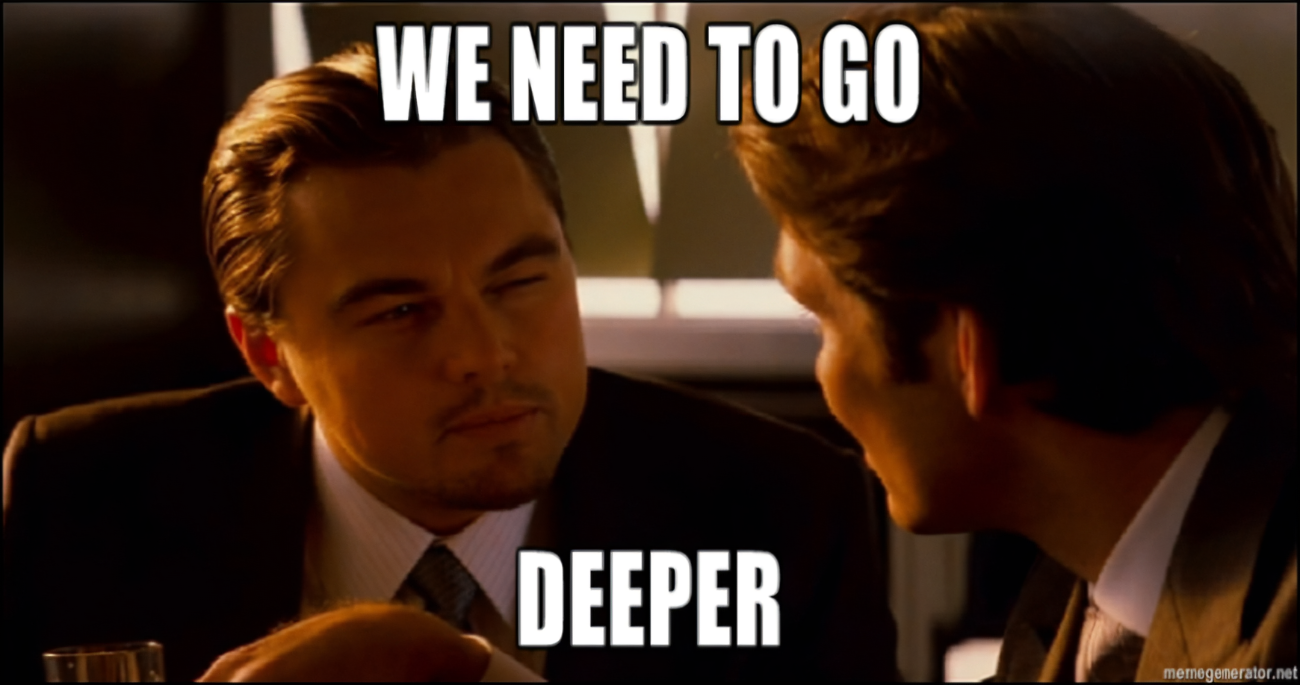
\includegraphics[width=0.5\linewidth]{godeeper.png}
                \caption{We need to go deeper, Inception}
                \label{fig:my_label}
        \end{figure}
    
\end{frame}

\begin{frame}[allowframebreaks]
    \bibliography{slides}
    \bibliographystyle{plain}
    % 如果参考文献太多的话,可以像下面这样调整字体:
    % \tiny\bibliographystyle{alpha}
\end{frame}

\begin{frame}
    \begin{center}
        {\Huge\calligra }
    
        {\Huge\calligra Thank you for your time!}
    \end{center}
\end{frame}

\end{document}